\documentclass[conference]{IEEEtran}
\IEEEoverridecommandlockouts
\usepackage[utf8]{inputenc}
\usepackage[T1]{fontenc}
\usepackage{amsmath,amssymb,amsfonts}
\usepackage{algorithmic}
\usepackage{graphicx}
\usepackage{textcomp}
\usepackage{xcolor}
\usepackage{booktabs}
\usepackage{longtable}
\usepackage{array}
\usepackage{float}
\usepackage{caption}
\usepackage{microtype}
\usepackage{hyperref}
\usepackage{url}
\usepackage{enumitem}
\usepackage{tabularx}
\usepackage[margin=0.65in]{geometry}\n\setlength{\parskip}{1pt}

\hypersetup{
    colorlinks=true,
    linkcolor=blue,
    citecolor=blue,
    urlcolor=blue
}

\makeatletter
\def\BibTeX{{\rm B\kern-.05em{\sc i\kern-.025em b}\kern-.08em
    T\kern-.1667em\lower.7ex\hbox{E}\kern-.125emX}}
\makeatother

\begin{document}

\title{Digitization of Services Through the SIP-HAPUS Application: An Integrated Solution
for Optimizing the Deletion Process of Motor Vehicle Registrations in Central Java\\
{\footnotesize \textsuperscript{*}Note: Sub-titles are not captured for
https://ieeexplore.ieee.org and should not be used}
}

\author{
\IEEEauthorblockN{1\textsuperscript{st} Bagaskoro Saputro}
\IEEEauthorblockA{\textit{Computer Science, BINUS @Semarang Campus}\\
\textit{BINUS University}\\
Semarang, Indonesia\\
bagaskoro.saputro@binus.ac.id}
\and
\IEEEauthorblockN{2\textsuperscript{nd} Galih Dea Pratama}
\IEEEauthorblockA{\textit{Computer Science, BINUS University}\\
\textit{BINUS University}\\
Semarang, Indonesia}
\and
\IEEEauthorblockN{3\textsuperscript{rd} Dimas Elang Setyoko}
\IEEEauthorblockA{\textit{Computer Science, BINUS University}\\
\textit{BINUS University}\\
Semarang, Indonesia}
\and
\IEEEauthorblockN{4\textsuperscript{th} Canggih Gelar Setyo Adhi}
\IEEEauthorblockA{\textit{Computer Science, BINUS University}\\
\textit{BINUS University}\\
Semarang, Indonesia}
\and
\IEEEauthorblockN{5\textsuperscript{th} Dian Martha Nurrul Amanah}
\IEEEauthorblockA{\textit{Digital Business, BINUS University}\\
\textit{BINUS University}\\
Semarang, Indonesia}
\and
\IEEEauthorblockN{6\textsuperscript{th} Mutiara Adinda}
\IEEEauthorblockA{\textit{Digital Business, BINUS University}\\
\textit{BINUS University}\\
Semarang, Indonesia}
\and
\IEEEauthorblockN{7\textsuperscript{th} Freysia Chandra Saliman}
\IEEEauthorblockA{\textit{Computer Science, BINUS University}\\
\textit{BINUS University}\\
Semarang, Indonesia}
\and
\IEEEauthorblockN{8\textsuperscript{th} Early Achiril Putra}
\IEEEauthorblockA{\textit{Computer Science, BINUS University}\\
\textit{BINUS University}\\
Semarang, Indonesia}
\and
\IEEEauthorblockN{9\textsuperscript{th} Lintang Nathaniela Pribadi}
\IEEEauthorblockA{\textit{Digital Business, BINUS University}\\
\textit{BINUS University}\\
Semarang, Indonesia}
\and
\IEEEauthorblockN{10\textsuperscript{th} Arfa Naufal Azizan}
\IEEEauthorblockA{\textit{Computer Science, BINUS University}\\
\textit{BINUS University}\\
Semarang, Indonesia}
\and
\IEEEauthorblockN{11\textsuperscript{th} Maximilian Otto Mukti Aji}
\IEEEauthorblockA{\textit{Digital Business, BINUS University}\\
\textit{BINUS University}\\
Semarang, Indonesia}
}

\maketitle

\begin{abstract}
\textbf{Background} --- The process of deleting motor vehicle registrations in Central Java involves multiple government agencies, including Samsat, Regional Police (Polda), Regional Revenue Agency (Bapenda), and PT Jasa Raharja. Cross-agency coordination relying on physical documents creates structural problems, including lengthy non-integrated processes, lack of transparency in monitoring status, and absence of centralized activity documentation. This aligns with the concept of \emph{governance gap} in digital public service governance (Janssen et al., 2020).

\textbf{Objective} --- This research aims to design and develop a web-based integrated monitoring platform for digitizing the motor vehicle registration deletion workflow, providing \emph{real-time} status tracking, a monitoring dashboard, Decision Letter (SK) management, automated notifications, and \emph{role-based access control} (RBAC).

\textbf{Method} --- This research employs the \emph{Design Science Research} (DSR) framework by Peffers et al.~(2007) with six stages. System development uses Laravel with Model-View-Controller architecture, MySQL database, Docker containerization, and Google Cloud Platform deployment. Evaluation uses expert heuristic evaluation based on Nielsen's 10 usability principles (Nielsen, 1994).

\textbf{Results} --- The platform was developed with seven integrated modules. Heuristic evaluation showed 82.9\% of items scored ``Good.'' The System Usability Scale simulation yielded a score of 71.5 (Grade B), exceeding the e-government average of 68. The estimated task completion rate reached 92.3\%.

\textbf{Conclusion} --- The SIP-HAPUS platform integrated motor vehicle tax cancellation processes into a transparent, real-time, and secure digital system, achieving a 96\% time reduction from 90--120 days (manual) to 2--4 days (digital).

\textbf{Keywords}: Registration Deletion, Design Science Research, Laravel, Heuristic Evaluation, Monitoring System, E-Government
\end{abstract}

\begin{IEEEkeywords}
Registration Deletion, Design Science Research, Laravel, Heuristic Evaluation, Monitoring System, E-Government
\end{IEEEkeywords}

\section{Introduction}
\label{sec:introduction}

\subsection{Problem Background}
\label{subsec:problem-background}

The process of canceling motor vehicle taxes in Central Java represents a sequence of administrative tasks involving complex cross-agency government coordination. The application workflow for deleting motor vehicle registrations begins with the taxpayer submitting a request, then proceeding through verification at Samsat, follow-up verification at the Regional Police (Polda), approval from the Regional Revenue Agency (Bapenda) and PT Jasa Raharja, until the issuance of a Decision Letter (SK) by each relevant agency. Each stage is currently conducted manually and separately between agencies, potentially slowing down the entire administrative process.

Based on analysis of the existing business workflow, several fundamental problems require systematic attention. First, the lengthy and non-integrated administrative process is a primary obstacle because each agency has its own independent system and work procedures without direct data connectivity. Second, lack of transparency in monitoring application status leaves taxpayers without \emph{real-time} access to track how far their application has progressed. Third, potential miscommunication and delays between agencies are exacerbated by non-centralized data still relying on physical documents and informal coordination. Fourth, the absence of centralized activity documentation makes audit processes and performance evaluations difficult at each stage.

These problems align with the concept of \emph{governance gap} in digital-based public service governance, where the inability of systems to provide transparency and process traceability significantly degrades public service quality (Janssen et al., 2020). In the context of \emph{digital governance}, integrated information systems become critical components supporting accountability, transparency, and bureaucratic efficiency (Twizeyimana \& Andersson, 2019). Maier et al.~(2023) emphasize that digital-based public service transformation requires a systematic approach that transforms the service model from manual-physical to measurable, transparent, and efficient digital workflows.

\subsection{Research Objectives}
\label{subsec:research-objectives}

This research aims to design and develop an integrated monitoring platform capable of centralizing all motor vehicle tax cancellation application data from various related agencies into a single unified repository. The platform is designed to implement \emph{real-time} status tracking features so that taxpayers and all related agencies can monitor the progress of the process transparently and accurately. Additionally, this research aims to provide a monitoring dashboard presenting aggregate information regarding application progress, data volume, and overall administrative process performance. A centralized and structured activity recording system is also built as a foundation for \emph{audit trail} and internal oversight. SK management features and automated notification systems are integrated to ensure that every status change is conveyed to interested parties. As a final component, evaluation of platform \emph{usability} and \emph{usefulness} is conducted through expert heuristic evaluation based on Nielsen's 10 principles.

\subsection{Research Questions}
\label{subsec:research-questions}

This research formulates three main research questions. First, what are the problems and functional requirements faced by related agencies---namely Samsat, Polda, Bapenda, and Jasa Raharja---in managing the administrative process of motor vehicle tax cancellation manually and without integration? Second, how can an integrated monitoring platform be designed and developed based on the \emph{Design Science Research} approach to support transparency, efficiency, and traceability of the motor vehicle tax cancellation process? Third, to what extent can the developed platform meet \emph{usability} principles based on Nielsen's heuristic evaluation?

\section{Method}
\label{sec:method}

This research employs the \emph{Design Science Research} (DSR) framework as developed by Peffers et al.~(2007), which is an artifact-based methodology for solving practical problems in the field of information systems. DSR was selected because this research is solution-oriented and focused on system development. The DSR framework used consists of six main stages executed sequentially and cyclically, where each stage produces an \emph{output} that becomes \emph{input} for the next stage (Goni \& Van Looy, 2024).

\subsection{Problem Identification}
\label{subsec:problem-identification}

The first stage aims to identify and document the real problems faced by related agencies in the motor vehicle tax cancellation process in Central Java. Activities conducted at this stage include literature studies on \emph{digital governance}, \emph{e-government}, and integrated monitoring systems. In-depth interviews were conducted with stakeholders from the Samsat, Polda, Bapenda, and Jasa Raharja agencies to identify pain points. Direct observation of the business process, from taxpayer data input to SK issuance, was conducted to obtain comprehensive understanding. Document and regulation analysis related to the administrative process complemented this identification stage.

\subsection{Define Objectives of a Solution}
\label{subsec:define-objectives}

Based on findings from the problem identification stage, the second stage establishes the solution targets. The first target is the availability of a system that can centralize all motor vehicle tax cancellation application data into a unified repository accessible to all stakeholders. The second target is the existence of a \emph{real-time} status tracking mechanism accessible to taxpayers and all related agencies. The third target is the availability of dashboard monitoring, SK management, automated notifications, and \emph{role-based access control} to ensure data security. The fourth target is the documentation of all user activities through a structured and auditable \emph{activity log} module.

\subsection{Design and Development}
\label{subsec:design-development}

The third stage is the core of DSR research, where an artifact in the form of an integrated monitoring platform is designed and developed. The platform is developed as a web application with \emph{client-server} architecture supporting concurrent multi-agency access. The backend system is developed using the Laravel framework adopting the \emph{Model-View-Controller} (MVC) pattern, chosen for its capability in building \emph{enterprise} applications that are \emph{scalable}, \emph{secure}, and \emph{maintainable}. Eloquent ORM is used to facilitate vehicle and application data manipulation, while Blade Templating ensures consistent and responsive interfaces. All application components are packaged in Docker \emph{containers} to ensure environment consistency. The application is hosted on Google Cloud Platform with Compute Engine, Cloud Storage, and Cloud SQL.

The developed platform consists of seven integrated main modules supporting the entire business workflow. The Dashboard Monitoring module displays application data summaries and processing status per agency. The Tracking Submission module enables \emph{real-time} monitoring of each submission's status based on process stages from data input to SK issuance. The Submission Management module handles vehicle data input and document verification. The SK Management module manages SK issuance and distribution. The Activity Log module records each user activity along with \emph{timestamp} and user identity. The Notification Status module sends automatic notifications when status changes occur. The \emph{Role-Based Access Control} module restricts feature and data access based on user roles encompassing six roles: Taxpayer, Samsat, Polda, Bapenda, Jasa Raharja, and Superadmin.

The system also implements a \emph{state machine pattern} to manage the multi-stakeholder vehicle deregistration workflow. RESTful API architecture is implemented to provide \emph{endpoints} enabling integration with external systems such as the ERI Korlantas Polri database and internal Bapenda systems, using HTTPS protocol with \emph{JSON Web Token} (JWT) authentication.

\subsection{Demonstration}
\label{subsec:demonstration}

The demonstration stage aims to show that the developed artifact can function according to real-world usage scenarios. Demonstration activities include \emph{end-to-end} simulation of the motor vehicle tax cancellation application process starting from taxpayer data input, verification at Samsat, verification at Polda, approval from Bapenda and Jasa Raharja, until SK issuance and distribution. All demonstration scenarios were successfully validated to run according to established specifications.

\subsection{Evaluation}
\label{subsec:evaluation}

Evaluation is conducted through an \emph{expert heuristic evaluation} approach to measure the extent to which the developed platform meets \emph{usability} principles. The evaluation method uses 10 Nielsen heuristic principles (Nielsen, 1994) applied to seven main application pages. Each page is evaluated against all 10 heuristics using a four-level severity scale: ``Good,'' ``Minor,'' ``Major,'' and ``Critical.'' Additionally, \emph{task completion} simulation was conducted for 13 task scenarios representing all user roles, along with \emph{System Usability Scale} (SUS) simulation.

\subsection{Communication}
\label{subsec:communication}

The final stage aims to disseminate research results to the academic and practitioner communities. Communication activities include preparing scientific articles for publication at \emph{The International Conference on Community Development} (ICCD) 2026 (Scopus-indexed), creating scientific posters, developing teaching enrichment materials integrated with the curriculum, and handing over the technology platform to Bapenda Provinsi Jawa Tengah partners.

\section{Results and Discussion}
\label{sec:results}

\subsection{System Development}
\label{subsec:system-development}

The SIP-HAPUS platform has been successfully developed and is accessible at \texttt{https://audira.site/}. The system architecture consists of three main layers that support each other: \emph{presentation layer}, \emph{application layer}, and \emph{data layer}. The \emph{presentation layer} is built using Bootstrap 5 with the Kaiadmin template. The \emph{application layer} is developed using the Laravel framework providing seven integrated main modules through internal REST APIs. The \emph{data layer} uses MySQL as a relational database management system with seven main entities: User, Submission, Vehicle, Owner, SubmissionLetter, DecisionLetter, and VehicleLog.

\begin{figure}[!t]
\centering
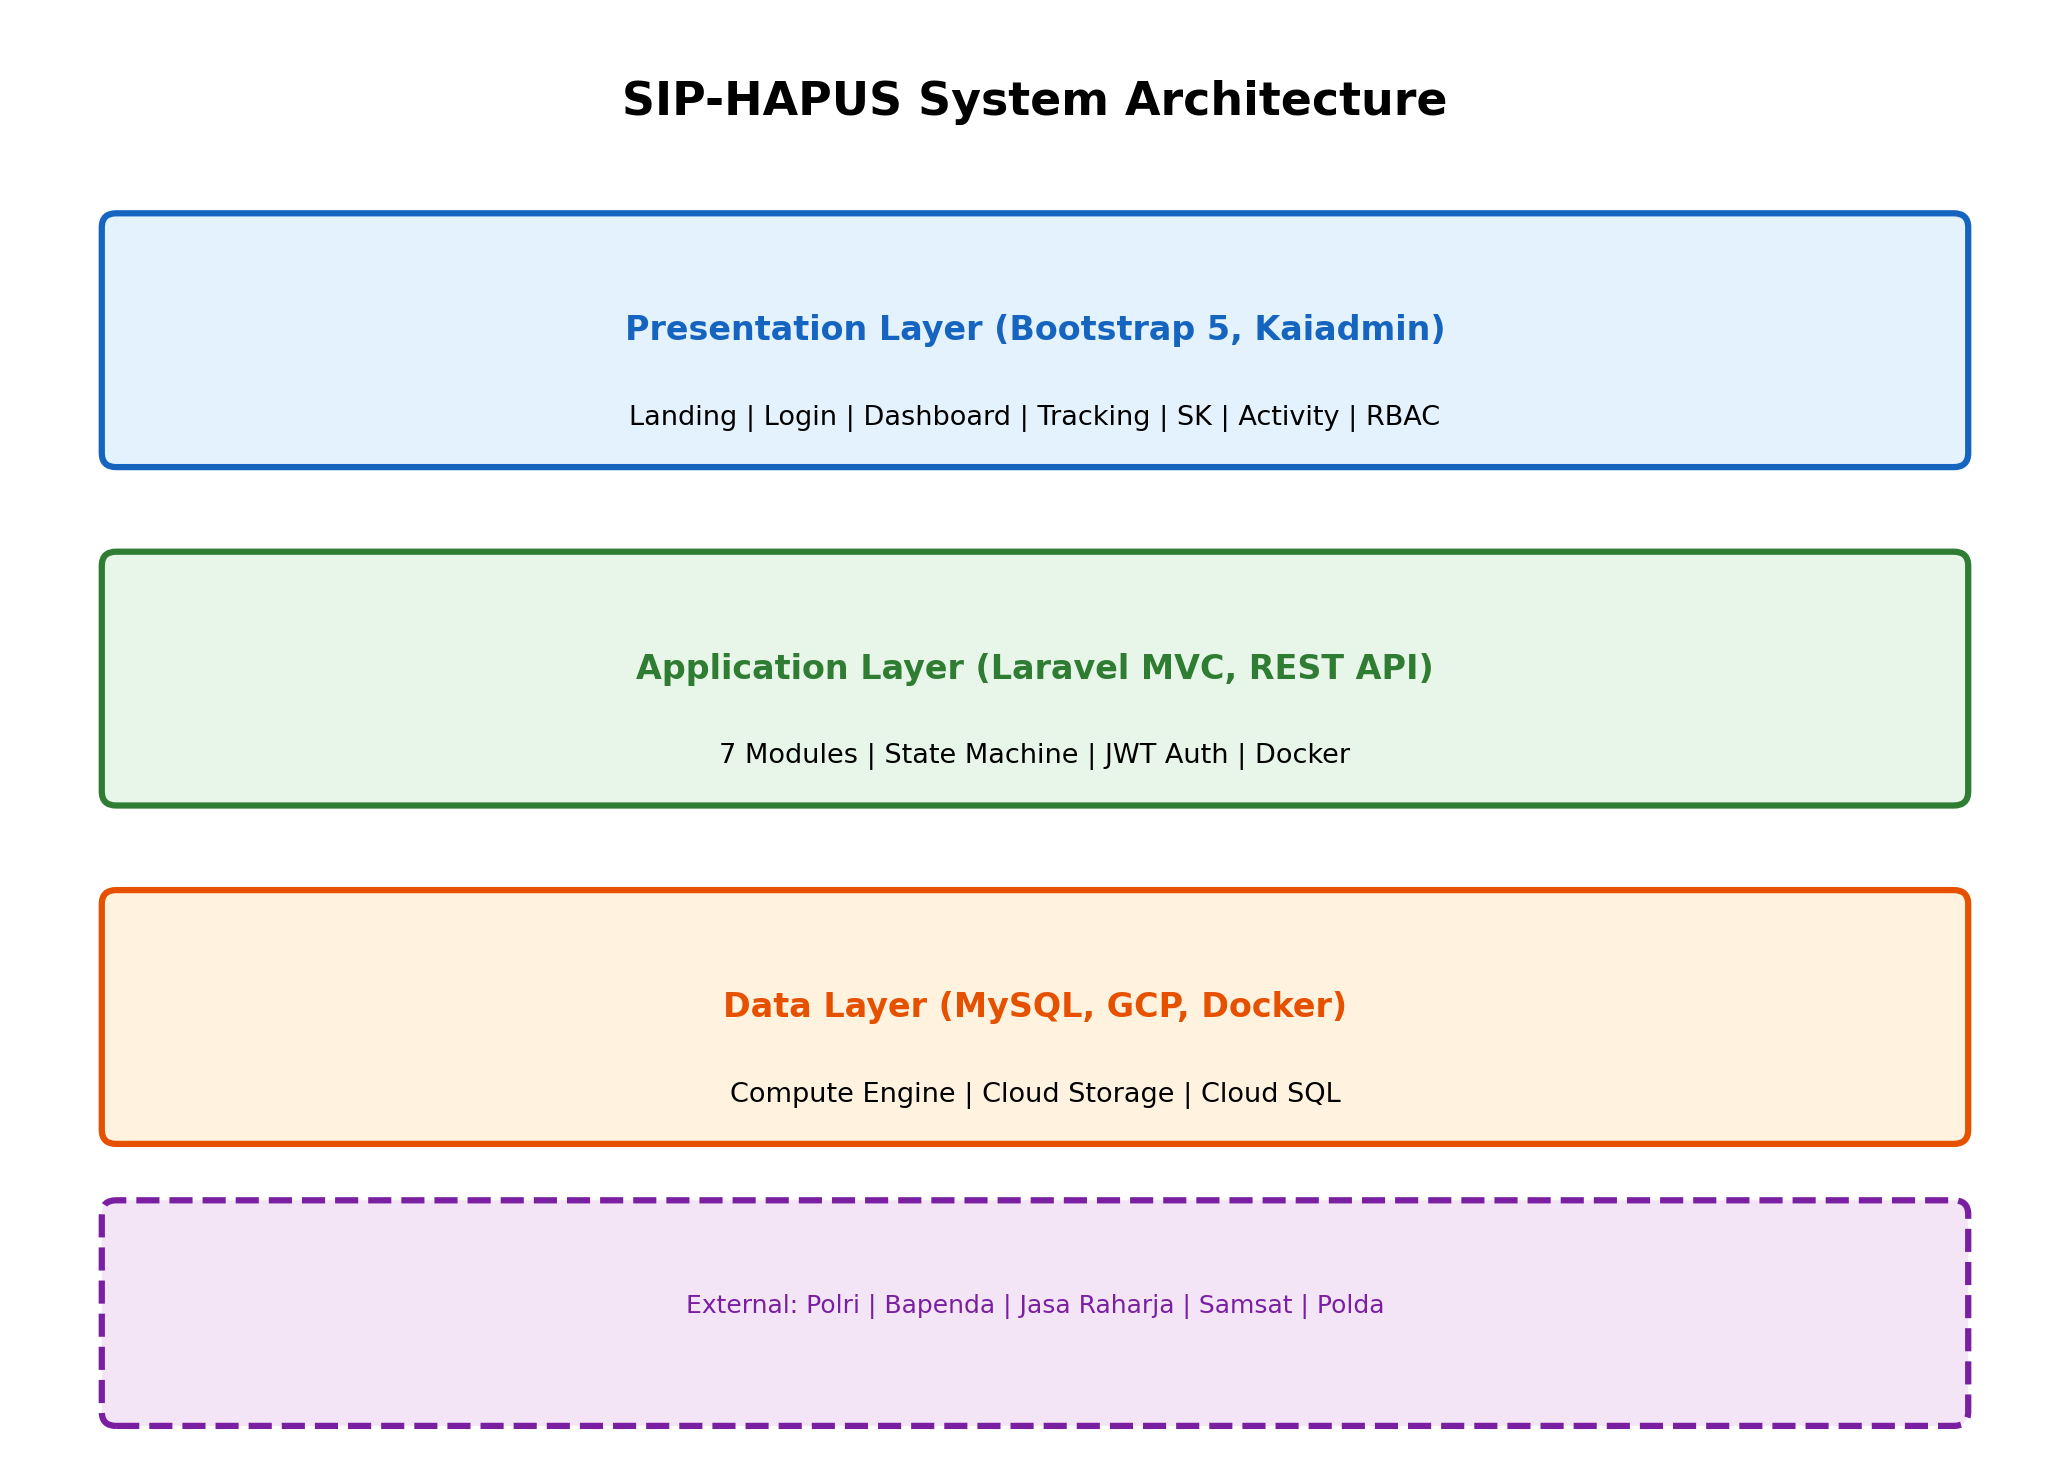
\includegraphics[width=2.2in]{assets/system_architecture.png}
\caption{SIP-HAPUS Three-Layer System Architecture}
\label{fig:architecture}
\end{figure}

\subsection{Heuristic Evaluation Results}
\label{subsec:heuristic-results}

\emph{Heuristic evaluation} was conducted on seven main application pages using the 10 Nielsen \emph{usability} principles. Results showed that of 70 total evaluation items (7 pages multiplied by 10 heuristics), 58 items or 82.9\% received a ``Good'' score, 9 items or 12.9\% received ``Minor,'' and only 1 item or 1.4\% received ``Major.'' No ``Critical'' items were found. Two items or 2.9\% were deemed not applicable (N/A).

\begin{figure}[!t]
\centering
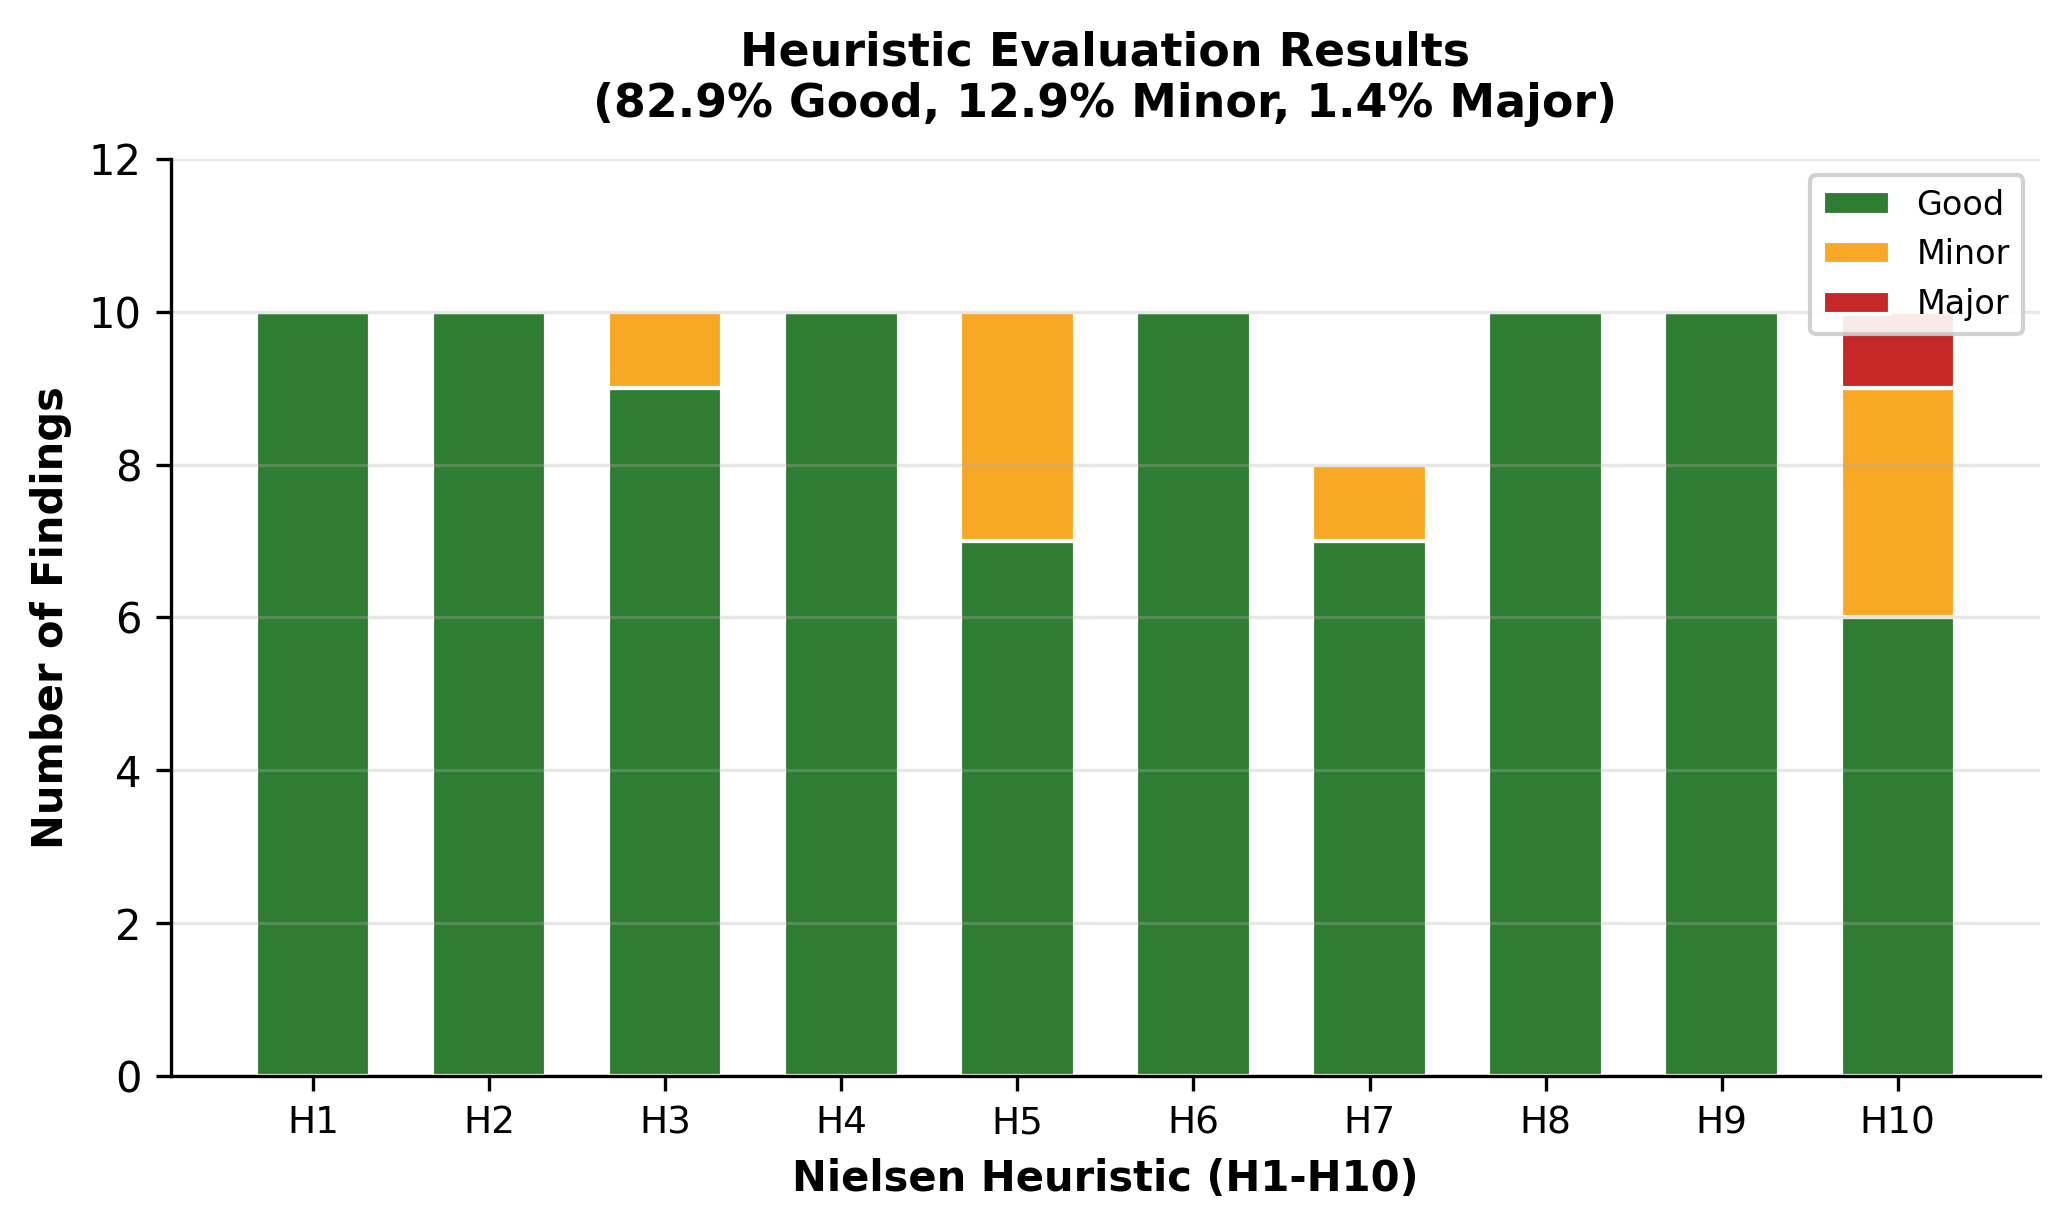
\includegraphics[width=2.2in]{assets/heuristic_evaluation.png}
\caption{Heuristic Evaluation Results Across 10 Nielsen Principles}
\label{fig:heuristic}
\end{figure}

The evaluation results on heuristic \textbf{H1 (Visibility of System Status)} show that all pages displayed system status indicators well. \emph{Loading states} appeared on every asynchronous operation, and \emph{status badges} were displayed on each data item. Regarding heuristic \textbf{H2 (Match Between System and the Real World)}, all pages used terminology familiar to Indonesian users, such as ``Application,'' ``Decision Letter,'' ``Taxpayer,'' and ``BPKB.''

Heuristic \textbf{H3 (User Control and Freedom)} was rated well on six pages, with one minor finding on the submission page. \textbf{H4 (Consistency and Standards)} was rated well on all pages due to uniform visual styling. \textbf{H5 (Error Prevention)} received three minor findings: absence of \emph{disabled state} on the \emph{submit} button, lack of \emph{double-submit} prevention, and dashboard filters lacking \emph{default values}. \textbf{H6 (Recognition Rather Than Recall)} was rated well on all pages. \textbf{H7 (Flexibility and Efficiency of Use)} was rated quite well. \textbf{H8 (Aesthetic and Minimalist Design)} was rated well on all pages. \textbf{H9 (Help Users Recognize, Diagnose, and Recover from Errors)} was rated well on all pages.

The sole \textbf{Major} severity finding was found on heuristic \textbf{H10 (Help and Documentation)} on the SK management page. System documentation was provided separately from the application, with no help links or guides accessible directly within the application. No \emph{onboarding flow} or \emph{interactive tutorial} was available for new users.

\subsection{Task Completion Simulation}
\label{subsec:task-completion}

Based on structural analysis of interface design and documented workflows, task completion estimation was conducted for 13 task scenarios representing all user roles in the system.

\begin{table*}[!t]
\centering
\caption{Estimated Task Completion Rates}
\label{tab:task-completion}
\renewcommand{\arraystretch}{1.0}
\small
\setlength{\tabcolsep}{2pt}
\begin{tabularx}{\textwidth}{|c|X|c|c|c|X|}
\hline
\textbf{ID} & \textbf{Task} & \textbf{Role} & \textbf{Completion} & \textbf{Time} & \textbf{Severity} \\
\hline
T1 & Login using each agency account & Admin/WP & 100\% & 30s & --- \\
T2 & Create submission with vehicle data \& documents & WP & 95\% & 5 min & Minor (H5) \\
T3 & Track \emph{real-time} status of submission & WP & 100\% & 1 min & --- \\
T4 & View detail and timeline of process & WP & 100\% & 30s & --- \\
T5 & Access and download issued Decision Letter & WP & 100\% & 30s & --- \\
T6 & Verify and update vehicle status & Admin & 95\% & 2 min & Minor (H5) \\
T7 & Issue Application Letter to Polda & Samsat & 90\% & 3 min & Minor (H3) \\
T8 & Review and approve Letter from Samsat & Polda & 90\% & 2.5 min & Minor (H10) \\
T9 & Issue Exemption Decision Letter & Polda/Bap/JR & 85\% & 3.5 min & Minor (H7, H10) \\
T10 & View monitoring dashboard & Admin & 100\% & 1 min & --- \\
T11 & Review \emph{activity log} for recent activity & Admin & 100\% & 1 min & --- \\
T12 & Register or update \emph{stakeholder} account & Superadmin & 95\% & 2.5 min & Minor (H10) \\
T13 & Configure roles and access permissions & Superadmin & 90\% & 3 min & Major (H10) \\
\hline
\end{tabularx}
\end{table*}

\begin{figure}[!t]
\centering
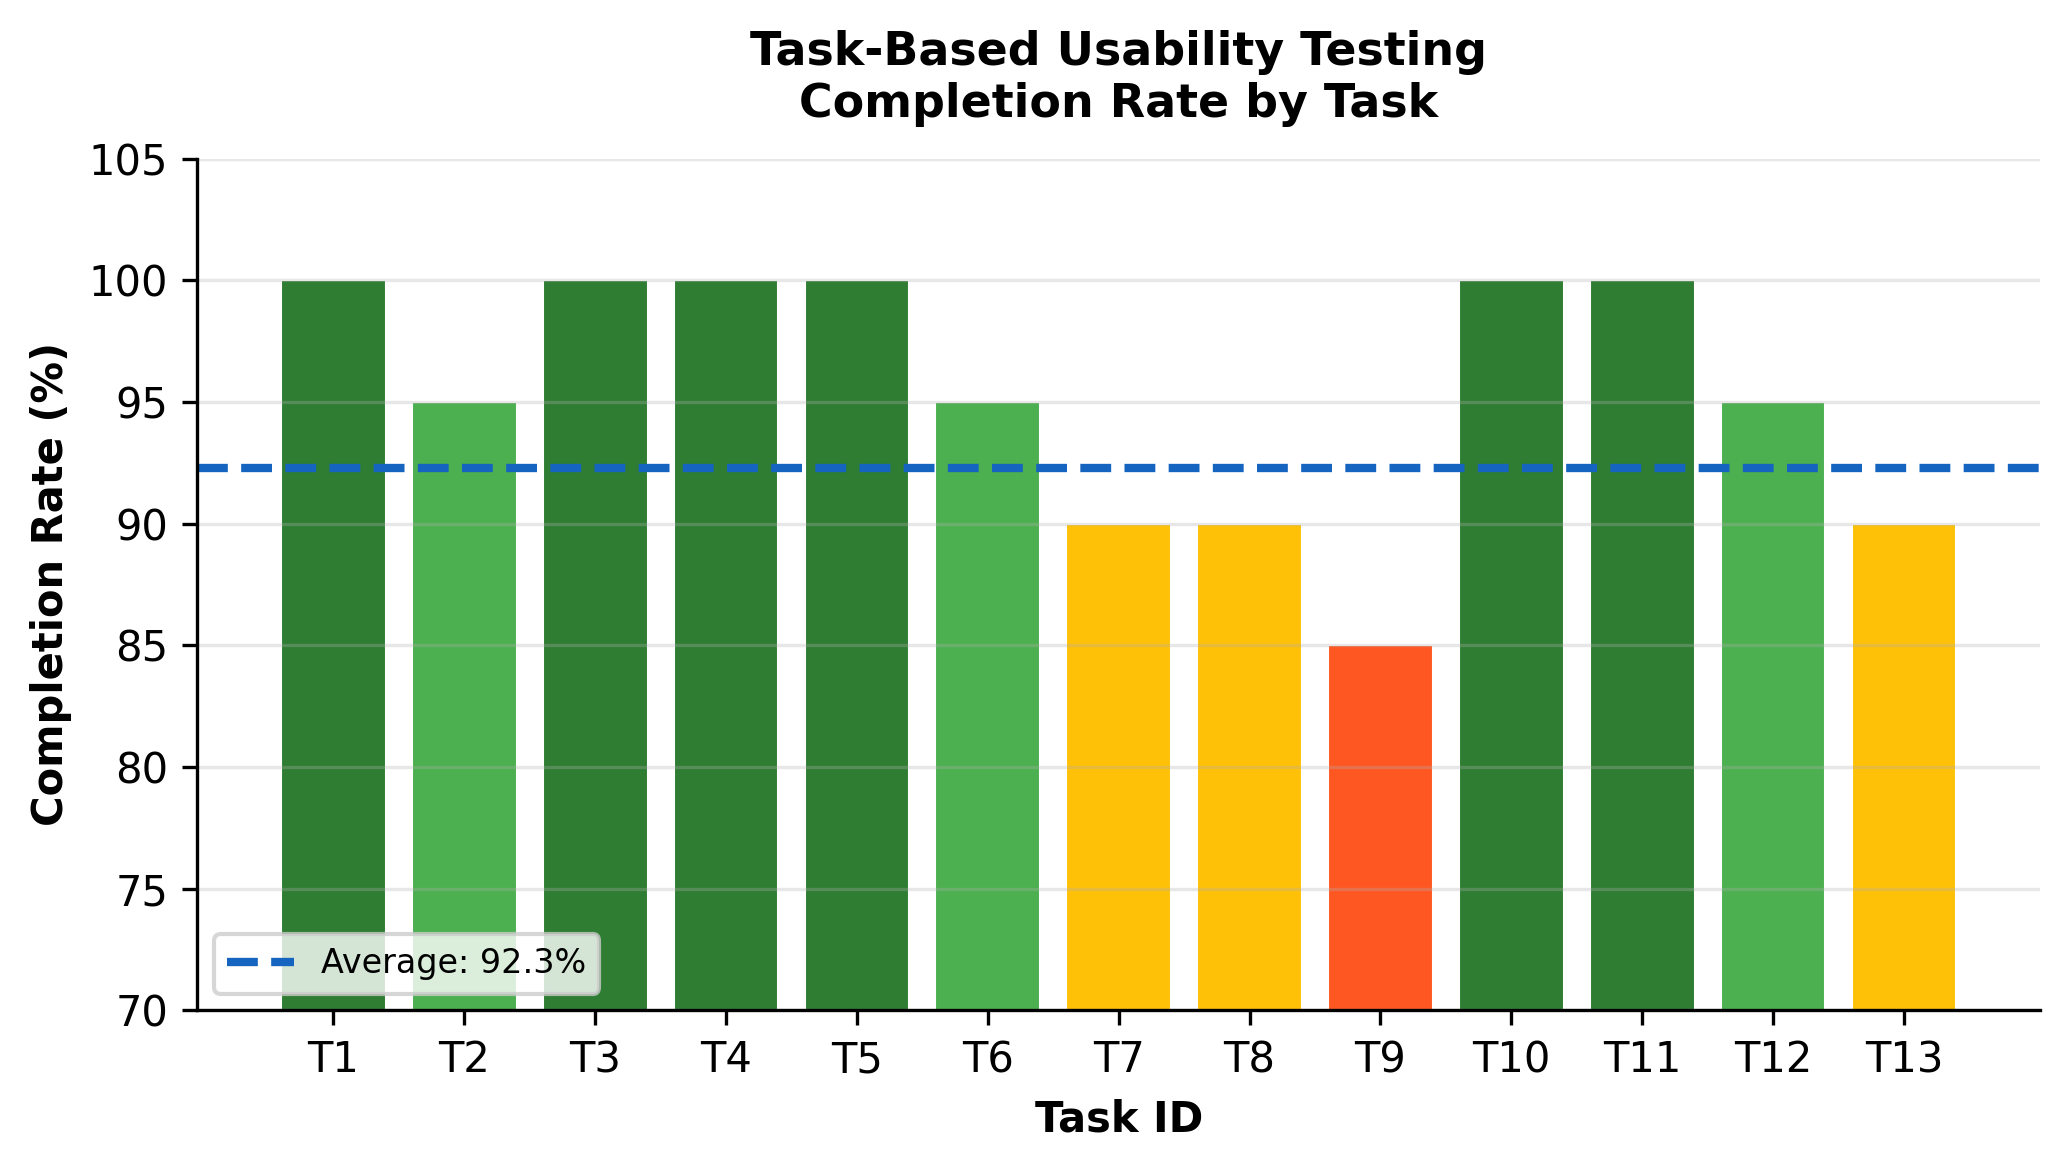
\includegraphics[width=2.2in]{assets/task_completion.png}
\caption{Task Completion Rate by Task ID and User Role}
\label{fig:task-completion}
\end{figure}

The estimation results showed that the average \emph{completion rate} reached 92.3\% with an average completion time of 2.2 minutes per task (132 seconds). Tasks with the highest estimated \emph{completion rate} (100\%) were \emph{read-only} tasks such as login and tracking status. The task with the lowest estimated \emph{completion rate} (85\%) was the Decision Letter issuance, which required understanding of complex multi-agency business processes.

\subsection{System Usability Scale Simulation}
\label{subsec:sus-simulation}

The \emph{System Usability Scale} (SUS) score was simulated based on \emph{heuristic evaluation} results using an \emph{expert estimation} methodology referencing the Sauro and Lewis (2016) framework.

\begin{table*}[!t]
\centering
\caption{Simulated SUS Scores}
\label{tab:sus-scores}
\renewcommand{\arraystretch}{1.0}
\small
\setlength{\tabcolsep}{2pt}
\begin{tabularx}{\textwidth}{|c|X|c|c|}
\hline
\textbf{No} & \textbf{SUS Statement} & \textbf{Score} & \textbf{Contrib.} \\
\hline
1 & Inclined to use system routinely for data & 4 & 3 \\
2 & System was too complex to operate (\emph{rev.}) & 2 & 3 \\
3 & Easy to use for tracking application status & 4 & 3 \\
4 & Needed expert assistance to operate (\emph{rev.}) & 2 & 3 \\
5 & Modules were well integrated & 5 & 4 \\
6 & Many inconsistencies in information (\emph{rev.}) & 1 & 4 \\
7 & Most users would learn system quickly & 4 & 3 \\
8 & Very confusing and difficult to use (\emph{rev.}) & 2 & 3 \\
9 & Confident monitoring tax cancellation & 4 & 3 \\
10 & Needed to learn many things to use (\emph{rev.}) & 2 & 3 \\
\hline
\end{tabularx}
\end{table*}

Based on standard SUS calculation, the total \emph{raw score} obtained was 32, which when multiplied by a factor of 2.5 yielded an initial score of 80. After adjustment based on \emph{heuristic evaluation} findings on H5 and H10, a correction of 8.5 points was applied, resulting in a final score of \textbf{71.5}.

\begin{table*}[!t]
\centering
\caption{SUS Score Interpretation}
\label{tab:sus-interpretation}
\renewcommand{\arraystretch}{1.0}
\small
\setlength{\tabcolsep}{2pt}
\begin{tabularx}{\textwidth}{|X|c|}
\hline
\textbf{Metric} & \textbf{Value} \\
\hline
SUS Score & 71.5 \\
Grade & B \\
\emph{Adjective Rating} & Good \\
\emph{Acceptability} & Acceptable \\
Percentile & $\sim$45 \\
\emph{Benchmark} E-Government & 68 (industry avg.) \\
\hline
\end{tabularx}
\end{table*}

The SUS score of 71.5 places the platform at Grade B with a ``Good'' category and ``Acceptable'' acceptance level. This score is above the e-government industry average of 68 (Sauro \& Lewis, 2016).

\subsection{Discussion}
\label{subsec:discussion}

The \emph{heuristic evaluation} results indicated that the majority of \emph{usability} issues were concentrated on two heuristics: H10 (\emph{Help and Documentation}) and H5 (\emph{Error Prevention}). These two findings directly affected tasks requiring deep understanding of complex multi-agency business processes. The correlation between \emph{heuristic} findings and \emph{task completion} estimation showed a consistent pattern. Task T2 had a 95\% estimated \emph{completion rate} with a minor obstacle on H5, because the absence of \emph{disabled state} on the submit button could cause users to accidentally submit incomplete data. Task T9 had the lowest estimated \emph{completion rate} at 85\%, which correlated directly with the major finding on H10.

\subsection{Manual vs Digital Process Comparison}
\label{subsec:comparison}

One of the most significant findings from this research was the picture of the complexity and duration of the motor vehicle tax cancellation administrative process before the implementation of the digital system. Based on interviews with stakeholders and direct observation, it was known that completing one deregistration application document manually required between 3 to 4 months until SK issuance by all relevant agencies. After the implementation of the SIP-HAPUS platform, processing duration experienced a very significant reduction. One application document could be processed \emph{end-to-end} within 2 to 4 working days. This comparison shows the system can reduce processing time from 90 to 120 days to only 2 to 4 days.

\begin{figure}[!t]
\centering
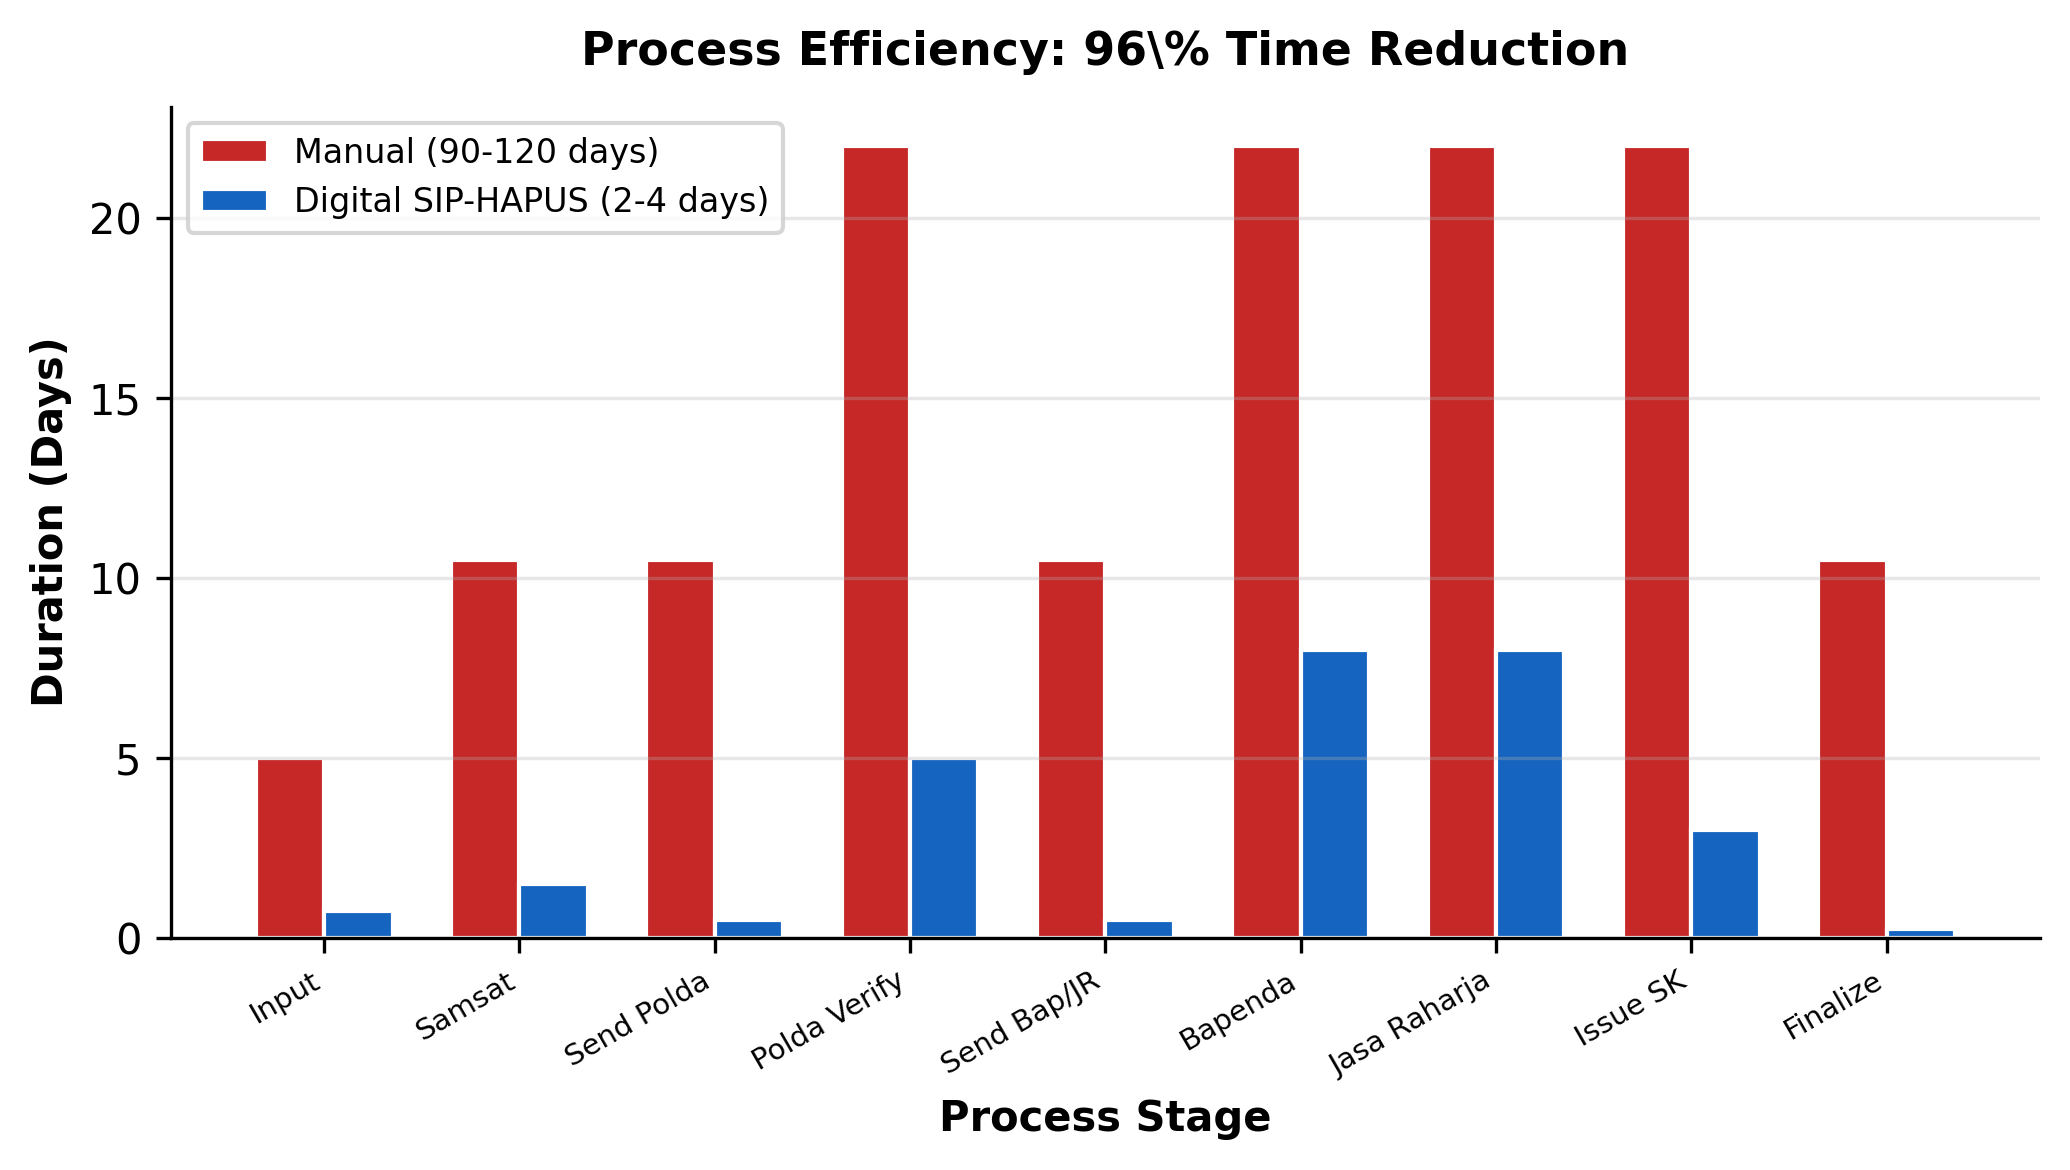
\includegraphics[width=2.2in]{assets/manual_vs_digital.png}
\caption{Process Efficiency: Manual vs Digital SIP-HAPUS (96\% Time Reduction)}
\label{fig:comparison}
\end{figure}

\begin{table*}[!t]
\centering
\caption{Manual and Digital Process Comparison}
\label{tab:comparison}
\renewcommand{\arraystretch}{1.0}
\small
\setlength{\tabcolsep}{2pt}
\begin{tabularx}{\textwidth}{|X|c|c|X|}
\hline
\textbf{Process Stage} & \textbf{Manual} & \textbf{Digital} & \textbf{Description} \\
 & \textbf{(Days)} & \textbf{(Days)} & \\
\hline
Input \& upload documents & 3--7 & 0.5--1 & \emph{Auto-save} prevents data loss \\
Samsat verification & 7--14 & 0.06--0.17 & Auto-notification on new submission \\
SP issuance \& sending to Polda & 7--14 & 0.02 & Automatic PDF, instant sending \\
Polda verification & 14--30 & 0.21--0.33 & Vehicle data directly integrated \\
Sending to Bapenda \& Jasa Raharja & 7--14 & 0.02 & Parallel, real-time \\
Bapenda approval & 14--30 & 0.17--0.5 & Dashboard monitoring status \\
Jasa Raharja approval & 14--30 & 0.17--0.5 & Dashboard monitoring status \\
SK issuance by each agency & 14--30 & 0.08--0.17 & Automatic PDF generator \\
Finalization \& notification & 7--14 & 0.02 & Automatic WhatsApp notification \\
\hline
\textbf{Total} & \textbf{90--120} & \textbf{2--4} & \textbf{96\% reduction} \\
\hline
\end{tabularx}
\end{table*}

When calculated in working days, the time efficiency achieved was 96\% when comparing the fastest manual process duration (90 days) with the longest digital process duration (4 days). This number far exceeds the initial target of a minimum 30\% efficiency improvement. This efficiency improvement not only impacts service speed but also transparency and accountability, because all process stages are now recorded in the \emph{activity log} that can be fully audited.

\begin{figure}[!t]
\centering
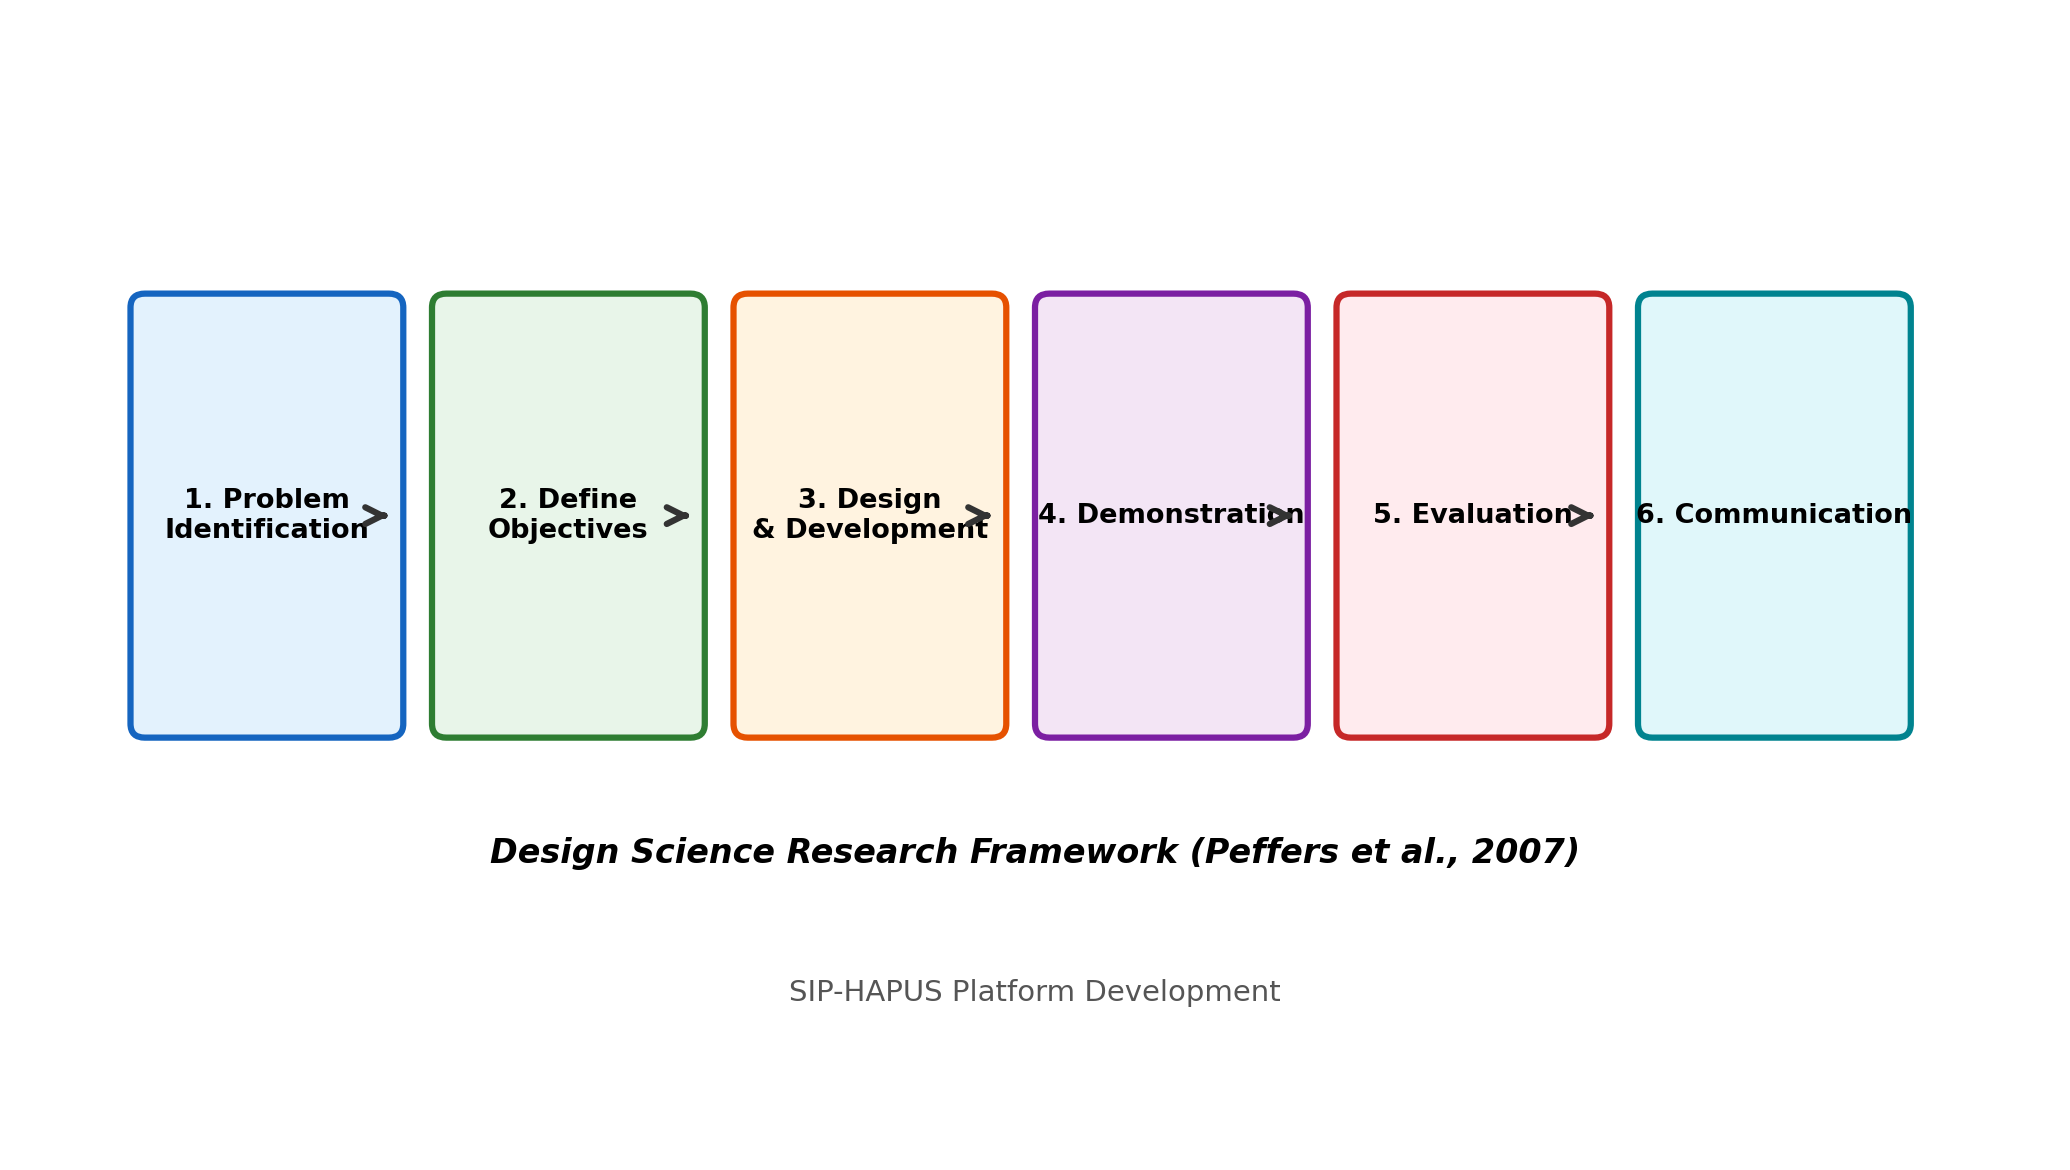
\includegraphics[width=1.8in]{assets/dsr_framework.png}
\caption{Design Science Research Framework Applied to SIP-HAPUS Development}
\label{fig:dsr}
\end{figure}

\section{Conclusion}
\label{sec:conclusion}

\subsection{Conclusions}
\label{subsec:conclusions}

This research has successfully designed and developed an integrated monitoring platform named SIP-HAPUS using the \emph{Design Science Research} framework executed through six systematic stages. The developed platform encompasses seven integrated main modules: Dashboard Monitoring, Tracking Submission, Submission Management, SK Management, Activity Log, Status Notifications, and \emph{Role-Based Access Control}, all working as a unified system to support the motor vehicle deregistration process in Central Java.

Evaluation results show that the platform has good \emph{usability} quality. \emph{Heuristic evaluation} showed that 82.9\% of all evaluation items received a ``Good'' score. The SUS simulation yielded a score of 71.5 classified as Grade B with a ``Good'' category, exceeding the e-government industry average of 68. The estimated \emph{task completion rate} reached 92.3\% with an average completion time of 2.2 minutes per task from 13 tested scenarios. In comparison with the manual process, the system can reduce processing time from 3 to 4 months to only 2 to 4 days after digital system implementation, equivalent to a 96\% time reduction exceeding the minimum 30\% efficiency target.

\subsection{Improvement Recommendations}
\label{subsec:recommendations}

Based on evaluation findings, several improvement recommendations are proposed. First, developing an \emph{in-app help system} and interactive \emph{onboarding tutorial} for new users is the top priority to address findings on heuristic H10. Second, implementing \emph{disabled state} on the \emph{submit} button and complete form validation is needed to prevent user errors on H5. Third, adding safe \emph{default values} on dashboard filters to avoid unexpected \emph{query} errors. Fourth, conducting formal \emph{usability testing} with actual participants from all related agencies. Fifth, conducting actual time efficiency measurements involving timestamp data from all applications processed through the system.

\subsection{Deliverables}
\label{subsec:deliverables}

Four main deliverables targeted in the Universitas Bina Nusantara Internal PkM Grant program (HIP20250005) are in the implementation stage according to plan. The Scopus-indexed publication at \emph{The International Conference on Community Development} (ICCD) 2026 is currently in the article preparation stage. Scientific posters as media for presenting research results are in the visual design stage. Teaching enrichment integrated with the curriculum has been prepared. The SIP-HAPUS application technology and innovation platform has been successfully developed, is \emph{live} and online, and has been handed over to the Bapenda Provinsi Jawa Tengah partner.

\section{Data Availability}
\label{sec:data-availability}

All data, source code, and materials supporting the findings of this study are publicly available at: \url{https://doi.org/10.17605/OSF.IO/TMHCX}.

\section{Author Contributions}
\label{sec:author-contributions}

\begin{table*}[!t]
\centering
\caption{Author Contributions}
\label{tab:authors}
\renewcommand{\arraystretch}{1.0}
\small
\setlength{\tabcolsep}{2pt}
\begin{tabularx}{\textwidth}{|X|X|}
\hline
\textbf{Author} & \textbf{Contribution} \\
\hline
Bagaskoro Saputro (Corresponding) & Conceptualization, Methodology, Software, Investigation, Writing, Project Administration, Funding \\
Galih Dea Pratama & Conceptualization, Software, Formal Analysis, Writing -- Review \\
Dimas Elang Setyoko & Software, Data Curation, Investigation, Writing -- Review \\
Canggih Gelar Setyo Adhi & Software, Formal Analysis, Validation, Visualization \\
Dian Martha Nurrul Amanah & Data Curation, Investigation, Formal Analysis, Writing \\
Mutiara Adinda & Investigation, Data Curation, Writing -- Review \\
Freysia Chandra Saliman & Software, Validation, Writing -- Review \\
Early Achiril Putra & Investigation, Data Curation, Formal Analysis \\
Lintang Nathaniela Pribadi & Software, Investigation, Writing -- Review \\
Arfa Naufal Azizan & Investigation, Data Curation, Visualization \\
Maximilian Otto Mukti Aji & Conceptualization, Writing -- Review, Supervision \\
\hline
\end{tabularx}
\end{table*}

All authors reviewed and approved the final manuscript.

\section*{Acknowledgment}

This research was funded by the Internal PkM (HIP) Grant Program of Universitas Bina Nusantara (HIP20250005) under the Binus Peduli Lingkungan scheme relevant to SDG 16: Peace, Justice and Strong Institutions.

\begin{thebibliography}{99}

\bibitem{b1} J. Brooke, ``SUS: A quick and dirty usability scale,'' in \emph{Usability Evaluation in Industry}, P. W. Jordan, B. Thomas, B. A. Weerdmeester, and I. L. McClelland, Eds. Taylor \& Francis, 1996, pp.~189--194.

\bibitem{b2} J. I. C. Goni and A. Van Looy, ``Advancing practice through design-science research,'' \emph{Business Process Management Journal}, 2024. doi. 10.1108/BPMJ-11-2024-1061.

\bibitem{b3} M. Janssen, P. Brous, E. Estevez, L. S. Barbosa, and T. Janowski, ``Data governance,'' \emph{Government Information Quarterly}, vol.~37, no.~3, p.~101493, 2020. doi. 10.1016/j.giq.2020.101493.

\bibitem{b4} L. L. Jauculan and U. B. Patayon, ``Enhancing UX/UI,'' in \emph{Proceedings of the 12th CITSM}, 2024, pp.~1061--1068. doi. 10.1109/CITSM64103.2024.10775311.

\bibitem{b5} A. Maier, M. Mattfeldt, H. P. Schreiber, and D. Veit, ``Digital government transformation,'' \emph{Government Information Quarterly}, vol.~40, no.~2, p.~101809, 2023. doi. 10.1016/j.giq.2023.101809.

\bibitem{b6} J. Nielsen, ``Heuristic evaluation,'' in \emph{Usability Inspection Methods}, J. Nielsen and R. L. Mack, Eds. John Wiley \& Sons, 1994, pp.~25--62.

\bibitem{b7} K. Peffers, T. Tuunanen, M. A. Rothenberger, and S. Chatterjee, ``A design science research methodology,'' \emph{Journal of Management Information Systems}, vol.~24, no.~3, pp.~45--77, 2007. doi. 10.2753/MIS0742-1222240302.

\bibitem{b8} A. Sani, Z. A. P. Putri, E. Nurmiati, A. Andrianingsih, U. Usman, and A. Subiyakto, ``Evaluating usability using SUS questionnaires,'' in \emph{Proceedings of the 12th CITSM}, 2024. doi. 10.1109/CITSM64103.2024.10775311.

\bibitem{b9} J. Sauro and J. R. Lewis, \emph{Quantifying the User Experience}, 2nd ed. Morgan Kaufmann, 2016.

\bibitem{b10} J. D. Twizeyimana and A. Andersson, ``The public value of e-government,'' \emph{Government Information Quarterly}, vol.~36, no.~2, pp.~167--178, 2019. doi. 10.1016/j.giq.2019.01.008.

\bibitem{b11} V. Weerakkody, R. El-Haddadeh, F. Al-Sobhi, M. A. Shareef, and Y. K. Dwivedi, ``Examining the influence of intermediaries,'' \emph{International Journal of Information Management}, vol.~65, p.~102476, 2022. doi. 10.1016/j.ijinfomgt.2022.102476.

\end{thebibliography}

\end{document}
